
% this file is called up by thesis.tex
% content in this file will be fed into the main document

%: ----------------------- introduction file header -----------------------


%------------------------------------------------------------------------- 


% the code below specifies where the figures are stored
\ifpdf
\graphicspath{{Sota/figures/PNG/}{./figures/}{Sota/figures/PDF/}{Sota/figures/}}
\else
\graphicspath{{Sota/figures/EPS/}{Sota/figures/}{./figures}}
\fi

\newcommand{\papersWithNumStudentInfo}[0]{103 }
\newcommand{\papersWithEvaluation}[0]{65 }
\newcommand{\hardwareHMD}[0]{8 }
\newcommand{\papersAfterTwentyEighteen}[0]{104 }
\newcommand{\allPapers}[0]{3070 }
\newcommand{\duplPapers}[0]{395 }
\newcommand{\papersCheckAbstract}[0]{2675 }
\newcommand{\papersToRead}[0]{359 }
\newcommand{\papersExludedAfterReading}[0]{228 }
\newcommand{\papersSelected}[0]{131 }
\newcommand{\papersMultiuser}[0]{23 }
\newcommand{\papersCollab}[0]{16 }
\newcommand{\papersGames}[0]{17 }

\chapter{Related Work}
\chaptermark{Related Work}
\label{chap:sota}

This Chapter presents a systematic review of the literature on the use of AR \mbox{applications} in primary and secondary schools, with a specific focus on collaborative, multi-user and interactive applications. It is based on a paper that included information up to the end of 2020 \citep{10.3897/jucs.76535}. The work is now updated with papers published as of September 2023. This study synthesises a set of 131 publications since 2015 and performs a qualitative analysis of their content. The review describes the current state-of-the-art of research in AR and presents the trends for the future of AR \mbox{applications} in educational settings, analysing the relevance of the multi-user interaction challenge within the augmented reality ecosystem.

\section{Overview} \label{sota:overview}
Digital transformation is profoundly impacting and disrupting every facet of society, and education is no exception. In recent decades, \gls{ar} has broken into the educational area. Nowadays, thanks to the widespread adoption of devices that support \gls{ar} applications, as well as the availability of software libraries such as ARKit or ARCore which greatly simplify and speed-up the development process, \gls{ar} has become a technology which is being more and more used in educational settings. Given its surge in popularity, AR has become an active research topic and several systematic studies have been performed to analyse how this technology has been used in educational contexts.

Some studies presented an analysis of the advantages and drawbacks of \gls{ar} in generic educational settings \citep{akccayir2017advantages, radu2014augmented, diegmann2015benefits} or have provided insights on the status of the technology, the availability of authoring tools as well as suggestions for future research \citep{cheng2013affordances, arici2019research, bacca2014augmented, pellas2019augmenting, dengel2022review}. Other reviews have focused on specific subjects, such as \gls{stem} \citep{ibanez2018augmented, nielsen2016augmented, ahmad2020augmented, sirakaya2022augmented} or language learning \citep{majid2021systematic, khoshnevisan2018augmented}; on specific topics such as \gls{ar}-based serious games \citep{li2017augmented, bartolome2011can, laine2018mobile}, the evaluation of the usage of \gls{ar} in schools \citep{da2019perspectives, chen2017review} or the impact of \gls{ar} applications in learning effectiveness \citep{garzon2019systematic, chang2022ten}. Table~\ref{tab:slrsummary} summarises the content of some of the most recent and comprehensive \glspl{slr} about \gls{ar} in educational settings.

\begin{table*}[htbp]
\caption{\fontsize{10pt}{11pt}\selectfont{\itshape{Summary of \glspl{slr} about usage of AR in education.}}}
\label{tab:slrsummary}
\small
\begin{tabular}{M{2.7cm}M{2.9cm}M{1.2cm}M{4.7cm}}
    \toprule
         \textbf{Study} & \textbf{Purpose} & \textbf{Papers} & \textbf{Findings} \\
    \midrule
         \cite{chang2022ten} & Investigate the impact of using AR apps in education & 134 & AR showed a medium effect to promote students’ positive responses to the learning experience, a medium to large effect to enhance students’ knowledge and skill, and a nearly large effect to facilitate students’ authentic performance \\
    \midrule     
          \cite{avila2021augmented} & Bibliometric analysis of studies of AR in education from 1995 to 2020 & 3475 & The number of publications on AR in education is increasing, and the field is gaining momentum; the current emerging and trending research topics in AR in education are special educational needs, Industry 4.0, storytelling, 3D printing, mobile applications, and higher education \\
   \midrule 
        \cite{law2021augmented} & Analyse AR apps for education from a usability and UX perspective & 49 & There is a disconnect between HCI and TEL communities; there are no AR-specific UX evaluation methods; the learner age seems not a significant factor in determining the perceived usability and UX or the learning effect of AR apps \\
    \midrule
         \cite{sirakaya2022augmented} & Advantages and challenges of using AR for STEM education & 42 & Use of AR in STEM education supports the learning and teaching process; there are not enough studies to test the effect of AR according to individual students characteristics \\
    \bottomrule

\end{tabular}
\end{table*}

Since the publication of the seminal paper on collaborative \gls{ar} by \cite{billinghurst2002collaborative}, which first discussed how AR could be used to enhance online and offline collaboration, much progress has been made in providing collaborative tools for \gls{ar} applications. So far, the only study which explicitly evaluates the usage of collaborative \gls{ar} applications for education is \citep{6821833}, which reviews publications on the subject from 2000 to 2013. In light of the numerous advancements in AR technology over the past few years, it is relevant to analyse the current literature about collaborative AR applications in education. This Chapter examines how AR apps function as tools for enhancing collaboration among students, as well as between students and teachers. Additionally, the review aims to explore how multi-user interfaces contribute to facilitate cooperation and learning.

Cooperative learning, defined as the instructional use of small groups to promote students working together to maximise their own and each other's learning \citep{johnson1991cooperation}, has long been used as an educational approach to improve the learning and performance of the students \citep{johnson2008active, kuh2011piecing}. Technology can help foster collaboration among students, but their engagement depends on how much they can interact with the different tools. AR \textit{per se} is not a collaborative tool: it is up to researchers and developers to provide such functionalities in an AR-based educational application. The objective of this Chapter is to evaluate which publications described AR applications providing the following features:
\begin{itemize}
    \item \emph{Levels of interactivity}: The app should respond to the user input and let the student modify the app content using different interaction methods (which will be described in detail in Section \ref{sota:results:RQ1}.
    \item \emph{Multi-user functionalities}: More than one user at the same time can use the app and the actions of one user are directly reflected in the device of other users.
    \item \emph{Collaboration}: Besides being multi-user, a collaborative app engages its users to collaborate or compete to reach a goal or complete a task.
\end{itemize}
Furthermore, how the usage of these applications affected the engagement of the students and their academic performance is described. 

This Chapter provides an \gls{slr} of the \gls{ar} applications deployed in primary and secondary schools, with a particular focus on the collaborative, multi-user and interactive characteristics of such applications. Only the articles published from 2015 to 2023 are considered, since in 2015 the number of publications related to the application of \gls{ar} in education has seen a huge increase (as shown in Figure~\ref{fig:pappublbg}). Furthermore, only works with an audience comprised of primary or secondary students are included, since there are already several works which review the usage of AR in higher education, and because this study was conducted in the context of the ARETE H2020 European project, studying multi-user AR applications for primary and secondary schools.

\begin{figure}[htbp]
	\begin{center}
	\includesvg[inkscapelatex=false, width=\textwidth]{papers_over_years}
	\captionsetup{font=small}
	\caption{\fontsize{10pt}{11pt}\selectfont{\itshape{Numbers of papers published per year with topic ``augmented reality'' and ``education'' from 2003 to 2023.}}}
	\label{fig:pappublbg}
    \end{center}
\end{figure}

The \glspl{RQ} addressed are the following:
\begin{enumerate}[start=1,label={\bfseries RQ\arabic*:}]
    \item What collaborative, multi-user, interactive \gls{ar} applications have been used in an educational environment in primary or secondary schools?
    \item Is there a motivation for using these \gls{ar} applications as an educational tool? If so, what is it?
    \item How effective are these \gls{ar} applications at improving the knowledge of the students? How is this evaluated?
\end{enumerate}

The answers to these RQs will hopefully provide researchers information about the current landscape of how AR applications are used in primary and secondary schools, what  the motivation is for it and what effects AR has on the learning and retention skills. Understanding the potential of interactive and collaborative AR, as well as its limitations and the factors limiting its usage in schools, can hopefully provide information on how future applications should be designed and developed.

Besides answering these research questions, the different technologies used by such applications will also be discussed. For example, the hardware required (\gls{hmd}, tablet or smartphone), the way the system tracks information from the real world (marker-based, markerless, location-based), whether the application augments other senses beyond vision, and which design strategies (if any) have been used to make the applications accessible.

\section{Methods}\label{sota:methods}
For this review, the guidelines proposed by \cite{kitchenham2009systematic} were followed and the search was framed using the PICOC criteria \citep{petticrew2008systematic}:
\begin{itemize}
    \item \textbf{Population}: Applications, Developers.
    \item \textbf{Intervention}: Collaborative, multi-user and interactive \gls{ar} applications.
    \item \textbf{Comparison}: The results of the students in classes which use AR applications with classes that do not.
    \item \textbf{Outcome}: Effectiveness in increasing understanding of a topic.
    \item \textbf{Context}: Education, primary or secondary schools.
\end{itemize}

Once the research questions have been defined, the literature review is split into three steps: planning, conducting and reporting. The Parsifal\footnote{\url{parsif.al}} online tool was used to conduct the first two steps of the review while the third was performed using Google Forms\footnote{\url{https://forms.gle/D7NHktgfaRmAeWTS8}}, to collect the results in a spreadsheet. The results of the data collection, as well as the code used to generate the figures in this document, are available on Github\footnote{\url{github.com/Stocastico/AR\_SLR\_Paper}}.


\subsection{Study selection}
The aim of this phase is to select the papers which are relevant for the systematic review, define the inclusion and exclusion criteria, and to provide the categories for the analysis.
Publications were selected from IEEExplore, Scopus, Springer and ISI Web of Science, as these four digital libraries collect most of the research that is published in the area of technology enhanced learning. The search terms \emph{Augmented Reality}, \emph{Education} $\lor$ \emph{Learning}, \emph{Collaborative} $\lor$ \emph{Interactive} $\lor$ \emph{Multi-user}, \emph{Application} $\lor$ \emph{Evaluation} were used, with the aim to include only papers that could help address RQ1 and RQ3. For this work, only papers which appeared online from 2015 to the end of August 2023 were considered. The search returned \allPapers results, of which \duplPapers were marked as duplicates. The abstract of the remaining \papersCheckAbstract articles were read and, applying the inclusion and exclusion criteria specified below, \papersToRead articles were left to read. Finally, after reading these articles \papersExludedAfterReading further documents were discarded, thus \papersSelected studies were selected for the literature review.
Table \ref{tab:searchstring} summarises the selection process, specifying the search string used for each digital library as well as the number of papers returned, marked as duplicated and selected for the systematic review.

As inclusion criteria, the studies have the following requirements:
\begin{itemize}
    \item Were published from 01/01/2015 to 31/08/2023.
    \item Describe an AR application  which has actually been implemented.
    \item Have a target audience of primary and/or secondary school students.
\end{itemize}

The focus for selection is only on applications that were fully developed (and could then be evaluated). This decision was taken to limit the amount of studies to analyse, but led to the exclusion of other interesting articles such as the one from \cite{osypova2021improving}, which studies the AR features of GeoGebra\footnote{\url{https://www.geogebra.org/}}, or \citep{tumler2022multi}, which describes an approach to research on multi-user and multiplatform XR experiences.

The studies selected should also present interactive, multi-user or collaborative applications. This is because there is a broad amount of literature showing that students learn better when engaged with other children, or being involved in interactive activities compared with purely passive ones. Finally, the decision to limit the literature search to papers published after 2015 is to avoid including older publications, often using obsolete hardware with setups that cannot be reproduced easily. The exclusion criteria are the following:

\begin{itemize}
    \item The application described is not interactive, multi-user or collaborative.
    \item The paper does not describe an AR application.
    \item The paper describes an unrelated application (e.g. for museums or clinical training).
    \item The paper is not peer reviewed.
    \item The paper is not written in English.
\end{itemize}

\begin{figure}[ht!]	
	\begin{center}
	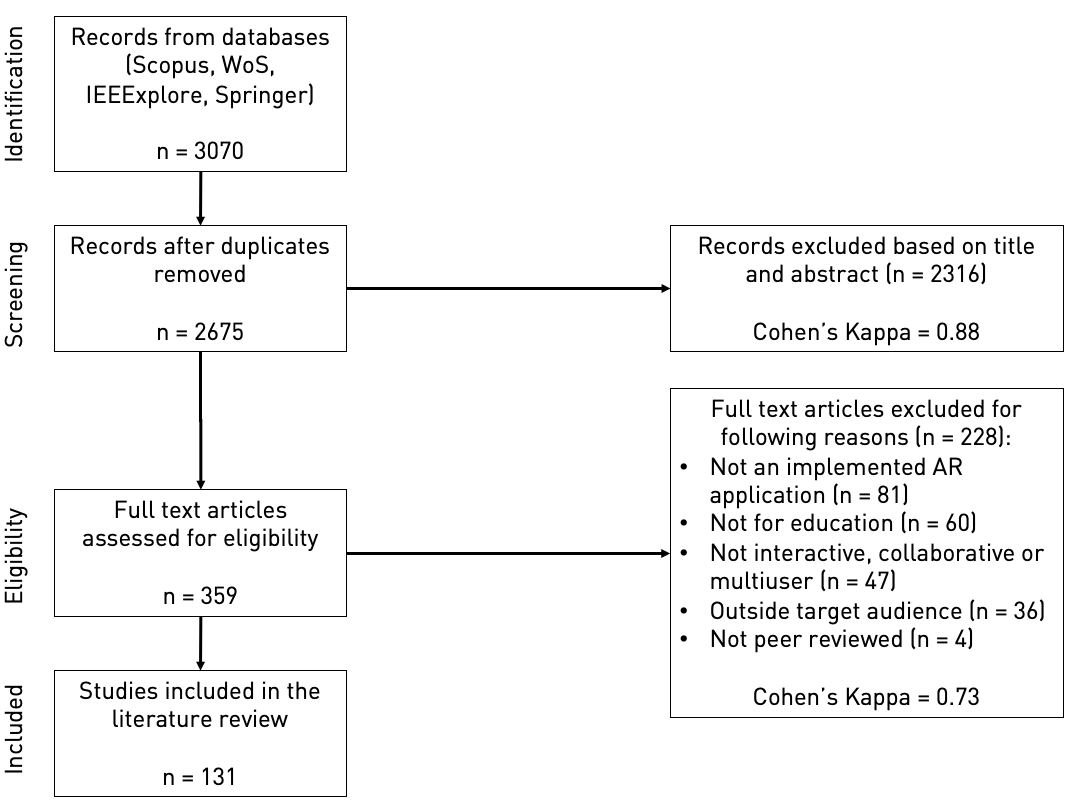
\includegraphics[width=\textwidth]{Prisma_flowchart.png}
	%\includegraphics[width=\textwidth]{figures/prisma_flowchart.png}
	\captionsetup{font=small}
	\caption{\fontsize{10pt}{11pt}\selectfont{\itshape{Prisma flowchart of the search protocol.}}}
	\label{fig:flowchart}
    \end{center}
\end{figure}

Figure \ref{fig:flowchart} shows a flowchart depicting the systematic review process. The \papersToRead papers were reviewed by 3 researchers. To compute the interrater agreement, two researchers read a set of 50 abstracts randomly selected from all the studies (excluding duplicates) and 10 papers (among the \papersToRead eligible papers). The interrater agreement, as defined in \cite{cohen1960coefficient} was $0.88$ for the abstracts and $0.73$ for the papers. The values represent\citep{mchugh2012interrater} an almost perfect agreement when selecting papers based on the abstract and a substancial agreement in the selection based on the whole text of the article. This indicates that the exclusion and selection criteria were defined in a clear, objective and replicable manner.


\begin{table}[!ht]
\caption{\fontsize{10pt}{11pt}\selectfont{\itshape{Query strings and number of papers returned.}}}
\label{tab:searchstring}
\small
\begin{tabular}{M{1.9cm}M{6cm}M{1cm}M{1.65cm}M{1.15cm}}
    \toprule
         \textbf{Digital Library} & \textbf{Query string} & \textbf{Papers} & \textbf{Duplicates} & \textbf{Selected} \\
    \midrule
         IEEExplore    &  (``All Metadata'': ``Augmented reality'' AND (``Education'' OR ``Learning'') AND (``Collaborative'' OR ``Interactive'' OR ``multi-user'' OR ``multi-user'') AND (``Application'' OR ``Evaluation'')) Filters Applied: 2015 - 2023 & 286 & 52 & \textbf{65} \\
    \midrule
        Scopus         & TITLE-ABS-KEY ( ``Augmented reality''  AND  ( ``Education''  OR  ``Learning'' )  AND  ( ``Interactive''  OR  ``multi-user''  OR  ``multiuser'' OR ``collaborative'' )  AND  ( ``Application''  OR  ``Evaluation'' ) )  AND  ( PUBYEAR $>$ 2014 )  & 963 & 196 & \textbf{118} \\
    \midrule
        Springer       & (collaborative OR interactive OR multiuser OR multi-user) AND ``augmented reality'' AND (education OR learning) AND (primary OR secondary) AND (application OR evaluation)
        within Chapter - Conference Paper  2015 - 2023  & 1289 & 88 & \textbf{99} \\
    \midrule
        Web of Science & ``Augmented reality'' AND (``Education'' OR ``Learning'') AND (``Collaborative'' OR ``Interactive'' OR ``multi-user'' OR ``multiuser'') AND (``Application'' OR ``Evaluation'') Filters Applied: 2015 - 2023 & 574 & 57 & \textbf{77} \\
    \bottomrule
\end{tabular}
\end{table}

\section{Results} \label{sota:results}

In this Section, the results of the three \glspl{RQ} introduced in Section \ref{sota:overview} are presented, focusing on the adoption of collaborative and multi-user tools, the advantages and disadvantages of using \gls{ar} solutions in the classroom and the evaluation of the interventions. The Section briefly analyses and summarises the main characteristics of the \gls{ar} applications described in the selected studies.

\subsection{Overview of reviewed studies}

Of \papersSelected studies reviewed, most of them (\papersAfterTwentyEighteen articles) were published in 2018 or afterwards. The vast majority of the AR apps analysed (88) cover STEM subjects, while 24 studies cover Humanities and Foreign language subjects. The remaining articles cover specific subtopics such as sustainability, creativity and social interactions or do not specify the subject. Figure \ref{fig:subjects} summarises the subjects covered by the AR apps analysed in this \gls{slr}.

\begin{figure}[htbp]	
	\begin{center}
	\includesvg[width=\textwidth]{subjects}
	\captionsetup{font=small}
	\caption{\fontsize{10pt}{11pt}\selectfont{\itshape{Subjects covered in the studies analysed.}}}
	\label{fig:subjects}
    \end{center}
\end{figure}


Regarding which AR type is used in the classroom, marker-based solutions (either image or QR-code based) are the most used, as two thirds of the studies described apps using markers as the exclusive source of the augmentations. 
Some studies describe applications using multiple types of \gls{ar}, usually a combination of markers and object detection based methods. Other types of \gls{ar} such as markerless or location based are seldom implemented, as they were used only in 10 and 3 articles, respectively. Figure \ref{fig:artech} summarises the types of AR used by the articles analysed in this \gls{slr}.

\begin{figure}[htbp]	
	\begin{center}
	\includesvg[width=\textwidth]{AR_technology}
	\captionsetup{font=small}
	\caption{\fontsize{10pt}{11pt}\selectfont{\itshape{Different types of AR used in the studies analysed.}}}
	\label{fig:artech}
    \end{center}
\end{figure}

With reference to the hardware required to experience the AR apps and the software used to develop them a similar pattern can be inferred. Most of the studies describe apps which have been developed for smartphones or tablets using the Unity\footnote{\url{unity.com/}} framework, often in conjunction with the Vuforia\footnote{\url{developer.vuforia.com/}} \gls{SDK}. Some studies, usually the oldest ones, describe systems using projectors or PCs with depth sensor cameras such as Microsoft Kinect\footnote{\url{developer.microsoft.com/en-us/windows/kinect/}}. Only \hardwareHMD articles describe apps which require \glspl{hmd} or smart glasses \citep{ oh2016designing, oh2017hybrid, matsutomo2017computer, khan2018mathland, wei2018improving, kum2019ar, radu2022augmented, resnyansky2022tangible}. This might be due to the higher cost of such devices and their consequent limited adoption compared to smartphones or tablets.

Using web technologies for the creation of AR application is still the exception rather than the norm: despite the availability of a javascript library such as Three.js\footnote{\url{threejs.org}} and frameworks such as A-Frame\footnote{\url{a-frame.io}}, only \cite{abriata2020building, protopsaltis2016quiz, rodriguez2021molecularweb} provide augmented content that can be consumed through the browser.
Somewhat surprisingly, very few studies rely on the libraries produced by Google and Apple (ARCore and ARKit), which were developed to provide advanced \gls{ar} functionalities for smartphone and tablets. A few studies \citep{carlos2021voluminis, costa2021interactive, acosta2020applying} have used ARCore in conjunction with Unity, but the current trend still favours less powerful but easier to use libraries such as Vuforia. Usage of specialised \gls{CV} libraries or \gls{DL} frameworks is also very low, which probably means that researchers prefer to use the functionalities provided by Unity. Statistics about software usage may be skewed, though, as about one fourth of the studies did not provide information about it.

Figures \ref{fig:hardware} and \ref{fig:software} summarise the hardware required and the software used by the apps analysed in this \gls{slr}. The total in this case does not sum up to \papersSelected since the same application could support more than one device and likewise it may have been developed using several software libraries.

\begin{figure}[htbp]	
	\begin{center}
	\includesvg[width=\textwidth]{Hardware_supported}
	\captionsetup{font=small}
	\caption{\fontsize{10pt}{11pt}\selectfont{\itshape{Device types supported by the AR applications.}}}
	\label{fig:hardware}
    \end{center}
\end{figure}

Unfortunately, researchers very rarely publish their code alongside their peer reviewed publication. Of all the studies analysed, only \cite{ManriqueJuan2017APA, laviole2018nectar, mylonas2019educational, abriata2020building, dominguez2022collaborative, farella2022arete, wellmann2022open} publicly released the source code of their applications. In some cases, the researchers published the application for free on Google Play or the App Store. Although, in principle, this allows other researchers to test the application, without releasing the source code this is impractical, as very rarely the application can be used without some form of adaptation (for example, translation of the content, inclusion of new multimedia elements or adjustments to the school curricula).

\begin{figure}[htbp]	
	\begin{center}
	\includesvg[width=\textwidth]{Software_used}
	\captionsetup{font=small}
	\caption{\fontsize{10pt}{11pt}\selectfont{\itshape{Software used to develop AR applications.}}}
	\label{fig:software}
    \end{center}
\end{figure}

\subsection{Interactive and collaborative capabilities of AR applications}\label{sota:results:RQ1}

This subsection addresses the first research question. Interactive, multi-user and collaborative capabilities of the \gls{ar} apps described in the selected studies were analysed. The studies were categorized into five different clusters, based on how the applications provide interactive functionalities. The categories were chosen by analysing the common traits of each study, as well as considering the characteristics of interactive applications in the context of education (assessment, feedback to the teacher, quizzes) and of user interface elements that enable the interaction. The five interactivity levels were defined as follows:

\begin{itemize}
    \item \emph{Basic interactivity}: The student can interact with the app through \gls{ui} elements such as menus and buttons directly in the augmented space.
    \item \emph{Object interaction}: the student can interact directly with the augmented content, without having to use \gls{ui} elements.
    \item \emph{Quiz}: The application provides quizzes (or allows teachers to add new ones) to test the understanding of a topic directly within the app, or it includes gamification concepts.
    \item \emph{Behaviour tracking}: The application keeps track of student behaviour and, using this information, the teacher can modify the content shown to the user. Both the active interactions (questions answered, buttons clicked) as well as passive usage of the app (time spent on each activity, for example) are logged and made available to the teacher so that the lecture can be modified accordingly.
    \item \emph{Augmented interactions}: The augmented content shown to the user may change depending on the interactions of the user with the environment, for example when changing the relative positions of different markers, or by varying the distance of the device from the markers.
\end{itemize}

In addition to these, \emph{multi-user} \gls{ar} experiences were considered. In these applications multiple students can view the same augmented content from different devices and any change, for example caused by the interactions of one of the students, is visible to all the other students as well.
Finally, \emph{collaborative} \gls{ar} applications are also of interest, that is applications where the students share a common goal and work together (or compete against each other) to reach it.

These applications are of particular interest because interactive learning environments have been shown to have a positive impact on the education of the students \citep{johnson2000animated}. At the same time, collaborative learning offers the students several benefits at the social, psychological, academic and assessment level \citep{laal2012benefits}. In Table \ref{tab:categorize_papers}, the \papersSelected articles reviewed were classified into the categories described above. Some of the studies can appear on multiple rows in the table, meaning that they may offer multiple interaction types as well as provide multi-user or collaboration functionalities. The works of \cite{tscholl2016designing} and \cite{ManriqueJuan2017APA} present collaborative application that were not categorised as multi-user, since only one device is shared by multiple students.

As it is impractical to provide a description of all the selected articles, a short description of the most interesting ones will be presented here. In \cite{khan2018mathland}, the authors implemented a mixed reality system based on HoloLens\footnote{\url{https://www.microsoft.com/en-us/hololens}} smart glasses and several stretch and \gls{IMU} sensors, where the users can control and move augmented objects using their arms or an ad-hoc controller. The multi-user application is used to teach the students physics concepts such as force fields or velocity vectors, without needing to set up a laboratory. Some studies use multiple markers to increase interactivity. The work of \cite{wang2018augmented} uses AR to teach the double-slit experiment (a physics experiment demonstrating the characteristic of light being both a wave and a particle). In the application each marker is related to one part of the experimental apparatus. By modifying the distance of each marker from the next one, the augmented animation generated by the app changes its behaviour, visually showing the dual nature of light. A similar idea is implemented by \cite{boonbrahm2015using}. In the app, which was created to facilitate learning English as a foreign language, each marker by itself only shows a letter in 3D. When multiple markers are combined to create an English word (from a predefined set), the app will show a 3D model of the corresponding word.

%\begin{table*}[t]
%\begin{center}
%\begin{tabular}{M{1.9cm}M{10.1cm}}
\fontsize{9}{11}\selectfont
{
\begin{longtable}[!t]{>{\raggedright\arraybackslash}p{0.15\textwidth}p{0.81\textwidth}}
\caption{\fontsize{10pt}{11pt}\selectfont{\itshape{Articles classified according to interactivity and collaboration capabilities.}}} 
\label{tab:categorize_papers} \\
    \toprule
    \textbf{Interaction type} & \textbf{Papers} \\
    \midrule
    \endhead
    Basic interactivity & \cite{lai2015applying, tang2015learning, ang2019enhancing, sorrentino2015speaky, arcos2016playful, zhao2018augmented, chao2018study, costa2019augmented, protopsaltis2016quiz, luna2018words, ramos2019artitser, el2019educational, huang2016animating, wang2017exploring, pombo2017marker, pombo2018edupark, chen2016augmented, liou2017influences, hsu2017learning, mylonas2019educational, khan2018mathland, hrishikesh2016interactive, sarkar2018scholar, chang2018impacts, chen2015construction, huang2019learning, lin2019primary, cao2018research, pombo2019learning, wei2019influence, cerqueira2018learning, klautke2018bridging, chang2019applying, hsieh2019intelligence, yilmaz2017using, lee2018augmented, chen2019effects, liu2020ar, perez2020interactive, yin2020research, mikulowski2020multi, korosidou2019gamifying, estudante2020using, 231-syahidi2020mobile, 232-cruzado2020idear, 236-9298003, 241-MACARIU20202133, 246-10.1145/3379350.3416155, 248-9339655, 251-10.1007/978-3-030-62655-6_9, resnyansky2022tangible, syamsudin2022development, sharma2022edusense, seel2022karli, xia2022development, buchner2021augmented, hossain2021augmented, debnath2021augmented, acosta2020applying, korosidou2021gamifying, dobrovska2021implementation, pasalidou2021teachers, carlos2021voluminis, adi2022pilot, uriarte2023comparison}\\
    \midrule
    Object interaction & \cite{arcos2016playful, costa2019augmented, iqbal2019exploring, cao2019hand, kum2019ar, cen2019augmented, ferrer2017virtual, oh2016designing, tscholl2016designing, laine2016designing, rusinol2018augmented, kurniawan2018human, boonbrahm2016interactive, ibanez2020impact, ManriqueJuan2017APA, chen2018application, mahmoudi2018color, antoniou2017scoping, hsu2018cobochild, thamrongrat2019design, lee2019mobile, amrit2015studies, ortiz2018evaluation, wei2018improving, rammos2019alternative, li2018see, giasiranis2017flow, takahashi2018empathic, lytridis2018artutor, matsutomo2017computer, kenoui2020teach, lopez2020emofindar, carlos2020voluminis, 231-syahidi2020mobile, 233-10.1145/3441000.3441034, 246-10.1145/3379350.3416155, 251-10.1007/978-3-030-62655-6_9, zhong2021design, radu2022augmented, dominguez2022collaborative, nabila2021mobile, farella2022arete, swearingen2021woods, logothetis2021transforming, cardenas2021yaniwawa, farella2021augmented, costa2021interactive, gargrish2022evaluation, rodriguez2021molecularweb, wellmann2022open}\\
    \midrule
    Quiz or gamification &  \cite{lai2015applying, costa2019augmented, protopsaltis2016quiz, ramos2019artitser, laviole2018nectar, limsukhawat2016development, lin2016effect, chang2018impacts, daineko2018development, pombo2019learning, lee2019mobile, ortiz2018evaluation, wei2018improving, li2018see, xefteris2019mixing, oh2017hybrid, dave2020towards, 232-cruzado2020idear, 233-10.1145/3441000.3441034, 241-MACARIU20202133, jumat2022augmented, dominguez2022collaborative, bakar2021gaar, el2021flcara, costa2021interactive}\\
    \midrule
    Behaviour tracking & \cite{protopsaltis2016quiz, chen2016augmented, mylonas2019educational, chang2018impacts, cao2018research, hsu2018cobochild}\\
    \midrule
    Augmented interaction & \cite{chao2018study, cen2019augmented, cai2017applications, ferrer2017virtual, wang2018augmented, laviole2018nectar, nasongkhla2019implementing, gardeli2018effect, xefteris2018learning, boonbrahm2015using, yilmaz2017using, kalpakis2018promoting, lam2020interactive, abriata2020building, dave2020towards, 241-MACARIU20202133, 251-10.1007/978-3-030-62655-6_9, el2021flcara, logothetis2021transforming, cardenas2021yaniwawa, gargrish2022evaluation, rodriguez2021molecularweb, wellmann2022open}\\
    \midrule
    Multi-user & \cite{kum2019ar, cai2017applications, oh2016designing, laviole2018nectar, boonbrahm2016interactive, gardeli2018effect, triantafyllidou2017fingertrips, xefteris2018learning, palaigeorgiou2018touching, lee2019mobile, ortiz2018evaluation, xefteris2019mixing, takahashi2018empathic, lee2018augmented, oh2017hybrid, dave2020towards, lopez2020emofindar, radu2022augmented, dominguez2022collaborative, farella2022arete, swearingen2021woods}\\
    \midrule
    Collaborative & \cite{cai2017applications, oh2016designing, tscholl2016designing, laviole2018nectar, boonbrahm2016interactive, ManriqueJuan2017APA, gardeli2018effect, lee2019mobile, ortiz2018evaluation, xefteris2019mixing, takahashi2018empathic, oh2017hybrid, lopez2020emofindar, dominguez2022collaborative, farella2022arete, swearingen2021woods}\\
    \bottomrule
\end{longtable}
}
\normalsize
%\end{tabular}
%\end{center}
%\end{table*}

In \cite{gardeli2018effect}, the students learn the basics of computer science by visually implementing algorithms. Each marker, besides showing augmented content, represents an instruction in ALGO, a specially developed programming language, and sequences of different markers generate different behaviour from the augmented content. \cite{241-MACARIU20202133}, implemented an app for learning Chemistry that includes a text recognition module to provide information on specific Chemistry-related words, as well as 3D animations that show the molecule created when combining different atoms, with each atom using a specific marker. In \cite{logothetis2021transforming}, the application implements hand-tracking technology that allows the students to directly modify the objects in the augmented space.

Only a few studies experiment with other senses beyond sight. The work of \cite{kenoui2020teach} uses the IBM Watson SDK\footnote{\url{www.ibm.com/cloud/watson-speech-to-text}} to allow the user to interact by asking questions in English, while the answer is shown both as text above the augmented content and as computer-generated audio. \cite{mikulowski2020multi} designed a system for visually impaired students that detects mathematical formulas and generates both an audio description as well as a Braille representation on the Braille display.
 
In the context of multi-user applications, different studies employed different strategies to foster collaboration. \cite{boonbrahm2016interactive} describe an application where the users aim to solve a jigsaw puzzle. Since students cannot move two pieces in a row but are forced to alternate their moves, the puzzle can only be solved with a joint collaboration. In the work of  \cite{ortiz2018evaluation}, the app is an \gls{ARGBL} where the user learns about different regions of Colombia while competing for resources. In this case, competition with others stimulate the students to learn about the subject. Another form of collaboration is described by \cite{oh2016designing}: the authors created a HMD-based AR application where the user can study properties of light such as reflection and refraction. Each user acts as a light source and sees what happens when light hits a wall or passes through different materials. At the same time, two or more users can generate multiple light rays and see how they interact with each other. Using a projector system, users without smart glasses are able to share the same experience, although not as actively as users wearing them. Another multi-user application for learning about electromagnetism is presented in \cite{radu2022augmented}, where multiple students can share the same experience in the augmented space.

Some applications incorporate functionalities to enable users to add new content. In \cite{costa2021interactive}, the AR application comes with a web application that allows to easily add new AR experiences, by specifying markers and their associate 3D objects. In \cite{wellmann2022open}, the authors prepared a repository with detailed instructions for creating new AR content, even though this is done in the form of Jupyter notebooks and thus require Python knowledge from the content creators.

\subsection{Motivation for using AR as an educational tool}

This subsection addresses the second research question. While the studies reviewed do not usually motivate the choice of the particular application presented in the articles, they do present however, several advantages provided by AR in the classroom. The main advantage provided by AR is that it can integrate seamlessly with the real world, especially for markerless applications that can interact with objects or printed material already available in the classroom. This encourages student engagement and minimises the time required to learn how to use the technology, allowing the students to spend more time learning the subject, as shown by \cite{thamrongrat2019design}. Another work by the same authors \citep{233-10.1145/3441000.3441034} shows that using gamification concepts in AR significantly impacts the students results.

Another advantage provided by AR is that this technology does not require the existing curriculum to be remodeled, rather it can be used as a tool to stimulate interest or to supplement existing pedagogical materials by simply adding more contextual experiences. \cite{pombo2018edupark} mention that using an AR app improves the engagement and interest of the students visiting an urban park by providing information that would otherwise be available only on textbooks.

AR is also a powerful tool for visualisation and animation, especially for STEM subjects, as it offers several advantages for displaying 3D or 3D+t information (i.e., three-dimensional data changing over time) in comparison to books, blackboards or videos. \cite{cao2019hand} describe an application for learning 3D geometry where the user can interact with 3D objects with their hands. The fingers are tracked with a Leap Motion Controller\footnote{\url{www.ultraleap.com/product/leap-motion-controller/}} while a set of markers are used to generate the augmented content. \cite{246-10.1145/3379350.3416155} use advanced features provided by ARKit (such as joint detection) together with object tracking technologies to provide interactions and visualizations through sketches drawn on the device.
In the context of collaborative and multi-user applications, AR similarly helps providing new opportunities for students to learn how to communicate and collaborate with one another, as well as to inspire empathy and to teach the importance of teamwork \citep{hill2013classroom}.

Some of the reviewed studies used AR applications as radically new tools that could improve skills and grades of children with mental or developmental disabilities: \cite{luna2018words} describe an application that helps students with \gls{ADHD} improve their English literacy skills. Similarly, \cite{chen2019effects} uses AR together with concepts maps to teach kids with \gls{asd} different types of social cues designed to help them when meeting people. \cite{takahashi2018empathic} designed a large scale AR and projection system, modifying the gymnasium of the school, to create a learning game for children with \gls{asd}, which intends to keep their attention focused on the content provided. Other studies, such as \cite{dominguez2022collaborative, farella2021augmented, farella2022arete} describe applications used in the context of \gls{pbis}, where the applications shows through examples and quizzes how to establish a positive student culture.

\cite{258-beyoglu2020use} check the effects of using mixed reality applications and how they impact the motivation of the students. They show that while such apps do not significantly impact the motivation to learn, they increase the motivation of the students for collaborative working, and the results are more significant for AR than for \gls{VR} apps. More in general, AR also compares favourably with respect to \gls{VR} not only because it allows users to perform tasks faster \citep{7833028}, but also because its requirements (namely a stable internet connection and one or more mobile devices), can be provided at a lower cost and the system does not need as much time to set up. Cost is often seen as one of the most important factors limiting the access of newer technologies, so in this sense AR is often seen as a better tool in comparison with VR or expensive hardware such as laptops and projectors.

\subsection{Effectiveness of collaborative AR applications}

This subsection addresses the third research question. Of the \papersSelected studies selected for this \gls{slr}, only \papersWithNumStudentInfo provided information about the number of students who tested the AR application. The number of students participating ranged from 2 to 290. Around 60\% of the studies were carried out with fewer than 40 participants and another 30\% were carried out with a number of participants between 41 and 80 students. Only 12 studies employed 100 or more students for the evaluation. Figure \ref{fig:testers} shows the histogram representing the distribution of users who tested the \gls{ar} application across the studies selected for review.

The analysis of the studies shows three main ways for evaluating how effective a \gls{ar} application can be in helping students improve their understanding of a subject: performing pre- and post- tests, comparing with a control group, and asking the teachers and/or the students to fill out surveys after the experiment.

\begin{figure}[htb!]	
	\begin{center}
	\includesvg[width=\textwidth]{hist_testers}
    \captionsetup{font=small}
	\caption{\fontsize{10pt}{11pt}\selectfont{\itshape{Histogram of the participant in user tests across different studies (grey) and its smooth density estimate (black).}}}
	\label{fig:testers}
    \end{center}
\end{figure}

While the first two options try to objectively measure the impact of using \gls{ar}, by analysing the grade of the students, the third option relies on the personal judgement of the teachers and students and can, in principle, be subject to bias.
In Table \ref{tab:cat_papers_evaluation}, the \papersSelected reviewed articles are classified into the categories described above. Some of the studies can appear on multiple rows in the table, meaning that they evaluate results of the students in more than one way. The table does not include studies in which no evaluation was performed, or in which surveys only asked about the app usability and ease of use.

\begin{table*}[ht!]
\small
%\begin{tabular}{M{2.7cm}M{2.9cm}M{1.2cm}M{4.7cm}}
%\begin{longtable}{p{0.15\textwidth}>{\arraybackslash}p{0.81\textwidth}}
\caption{\fontsize{10pt}{11pt}\selectfont{\itshape{Classification of studies according to the method used to evaluate the effectiveness of \gls{ar} in the classroom.}}}
\label{tab:cat_papers_evaluation} 
\begin{tabular}{>{\raggedright\arraybackslash}p{0.15\textwidth}p{0.81\textwidth}}
    \toprule
    \textbf{Evaluation type} & \textbf{Papers} \\
    \midrule
    Pre- and post- tests & \cite{lai2015applying, chao2018study, cao2019hand, el2019educational, cen2019augmented, huang2016animating, chang2018impacts, limsukhawat2016development, liou2017influences, laine2016designing, lin2016effect, ibanez2020impact, chen2018application, nasongkhla2019implementing, huang2019learning, lin2019primary, xefteris2018learning, pombo2019learning, thamrongrat2019design, ortiz2018evaluation, li2018see, chang2019applying, xefteris2019mixing, lee2018augmented, oh2017hybrid, chen2019effects, liu2020ar, carlos2020voluminis, korosidou2019gamifying, 231-syahidi2020mobile, 232-cruzado2020idear, 233-10.1145/3441000.3441034, 236-9298003, 241-MACARIU20202133, radu2022augmented, nabila2021mobile, carlos2021voluminis, cardenas2021yaniwawa, uriarte2023comparison, gargrish2022evaluation}\\
    \midrule
    Control group & \cite{arcos2016playful, cen2019augmented, huang2016animating, chang2018impacts, cai2017applications, hsu2017learning, hrishikesh2016interactive, sarkar2018scholar, thamrongrat2019design, ortiz2018evaluation, hsieh2019intelligence, yilmaz2017using, giasiranis2017flow, takahashi2018empathic, carlos2020voluminis, 232-cruzado2020idear, 233-10.1145/3441000.3441034, 236-9298003, hossain2021augmented, korosidou2021gamifying, carlos2021voluminis, uriarte2023comparison}\\ 
    \midrule
    Survey or interviews & \cite{costa2019augmented, luna2018words, ramos2019artitser, el2019educational, cen2019augmented, chang2018impacts, wang2017exploring, ferrer2017virtual, pombo2017marker, pombo2018edupark, chen2016augmented, oh2016designing, tscholl2016designing, wang2018augmented, mylonas2019educational, ManriqueJuan2017APA, chen2015construction, chen2018application, huang2019learning, mahmoudi2018color, gardeli2018effect, triantafyllidou2017fingertrips, xefteris2018learning, hsu2018cobochild, palaigeorgiou2018touching, pombo2019learning, ortiz2018evaluation, li2018see, hsieh2019intelligence, kalpakis2018promoting, oh2017hybrid, chen2019effects, 241-MACARIU20202133, 246-10.1145/3379350.3416155, 248-9339655, jumat2022augmented, syamsudin2022development, seel2022karli, xia2022development, buchner2021augmented, nabila2021mobile, el2021flcara, dobrovska2021implementation, pasalidou2021teachers, carlos2021voluminis, adi2022pilot, farella2021augmented, costa2021interactive, rodriguez2021molecularweb}\\
    %\hline
    % No evaluation & \cite{tang2015learning, ang2019enhancing, sorrentino2015speaky, zhao2018augmented}  \cite{iqbal2019exploring, protopsaltis2016quiz, kum2019ar, rusinol2018augmented, kurniawan2018human, khan2018mathland, laviole2018nectar, boonbrahm2016interactive, cao2018research, antoniou2017scoping, daineko2018development, lee2019mobile, boonbrahm2015using, amrit2015studies, wei2019influence, cerqueira2018learning, klautke2018bridging, wei2018improving, rammos2019alternative, lytridis2018artutor}\\
    \bottomrule
%\end{longtable}
\end{tabular}
\end{table*}

%\end{center}
%

It is worth mentioning the work described in \citep{chang2018impacts}. The researchers developed a system which, apart from the AR application, included a \gls{DBMS}, a teacher interface and an e-learning platform. The evaluation of the system includes a statistical analysis of the performance of the students and their learning achievements, as well as an analysis of the ease of use of the system for teachers and students. The application described in \cite{thamrongrat2019design} uses AR to teach children about 3D geometry. Pre- and post- tests were used along with quizzes to evaluate the system. The results showed that students who used the AR applications consistently had better grades than the control group, but such results were not statistically significant. Analysing the results for different tasks, however, the data showed that the group who used AR performed worse on the easiest task, while performing much better (with statistically significant results) than the control group in more complex tasks. From this, the authors concluded that AR can be a valuable tool for learning difficult geometric concepts. The same study also conducted tests about the user experience, and the results showed that the AR application could engage its users in extremely worthwhile, highly attractive and interesting learning activities with good usability.

The app described in \cite{cen2019augmented} is used to teach Chemistry to 45 high school students and behaves differently depending on the distance of the device from the markers. The authors performed a quantitative evaluation of the system, analysing the grades and the distribution of mistakes in the different quizzes. They concluded that there is a statistically significant improvement in the performances of the students, and that the greater the difficulty level of the question, the bigger the performance improvement is over the control group. The authors concluded that their Augmented Immersive Reality (AIR) system is most likely responsible for the bulk of learning improvements and the knowledge retention gains demonstrated in their case study, since that is the critical component differentiating their system from other applications available on the market.

Of the \papersWithEvaluation studies presenting a quantitative evaluation of the results, none of them concluded that using AR in the classroom has a negative impact on the results of the students and their level of engagement in the classroom. Even though, in many cases, the improvement over traditional teaching methods is limited, only \cite{carlos2020voluminis} do not detect any positive impact. This consensus on the effectiveness of AR applications is unexpected: besides the commonplace explication (AR is indeed a successful medium with a  positive impact on the results of the students) two other possible explanations are the novelty effect \citep{pisapia1993learning}, which explains the performance improvements introduced by a new technology such as AR as being due to an increased interest of the user, and the positive publication bias \citep{begg1994publication}, which makes it harder for researchers to publish studies with negative results.

Only \cite{lin2016effect, gargrish2022evaluation} present an analysis of the retention of the topics learned through \gls{ar} over a time span of more than two months. As most of the students who participated in the tests had not previously used \gls{ar} applications, there is a specific risk that the novelty effect introduced a recency bias, by increasing user engagement and knowledge acquisition, indirectly leading to better test scores.

\section{Discussion} \label{sec:discussion}
The research community is very active in investigating how \gls{ar} applications can improve education and facilitate understanding of difficult concepts.
Even though collaboration and participation by students is often seen as a key towards improving knowledge retention, there is still a lack of support for cooperation mechanisms in AR applications for education: of the \papersSelected studies analysed, only \papersMultiuser described multi-user application and only \papersCollab employ some sort of collaboration between users. \gls{ARGBL} is also quite uncommon, as only \papersGames articles describe applications which implement gamification concepts. 

By reviewing the existing literature, several issues that are preventing the widespread adoption of collaborative \gls{ar} in the classroom were identified:
\begin{itemize}
    \item \textit{Lack of authoring tools}: With the exception of \cite{lytridis2018artutor, whitlock2020mrcat, farella2021augmented, farella2022arete}, the applications described do not make use of an authoring tool that simplifies the creation of an AR experience. All the authoring tools presented in the aforementioned SLR from \cite{dengel2022review} are very limited and none of them offers a no-code solution. Other authoring tools presented in the literature \citep{rajaram2022paper, blattgerste2023trainar} have not been used in other studies. The lack of widespread, easy-to-use authoring tools requires every AR application to be developed from scratch. This leads to longer development times and more work required from the developers.
    \item \textit{Lack of standardisation for the description of AR experiences}: Of all the papers analysed, only \cite{farella2022arete} mentioned using a standard for the description of how AR is used in the application. This is mainly due to a lack of specific standards, as the IEEE ARLEM standard \citep{arlem2020} for AR-based learning experiences was only released in February 2020, while the ETSI Augmented Reality Framework\footnote{\url{www.etsi.org/committee/1420-arf}} document with AR authoring functions was published in August 2021. The adoption of these standards will drive and simplify the development of \gls{ar} applications for education, as well as foster interoperability.
    \item \textit{Availability of 3D content for education}: A few repositories where users can freely download 3D objects already exist, but there is a lack of 3D content specialised for education purposes. Although efforts have been made to solve the issue \citep{masneri2020work, deitke2023objaversexl}, this currently hinders the possibility of quickly and cheaply creating new AR apps for primary and secondary schools.
    %: very often the apps never leave the prototype stage and they are not turned into a fully-fledged product or used further in the classroom.
    \item \textit{Code publication}: Out of all the studies reviewed, only 7 provided the code of the \gls{ar} application, and only one \citep{wellmann2022open} provides detailed information on how to replicate and extend the work of the researchers. Not releasing the code as open source means that researchers cannot build upon the results of previous studies: even for the more interesting and highly cited articles there will be no follow up work, with the exception of that from the original authors.
\end{itemize}

Studies claiming to have a stronger positive impact on educational achievements are the ones where the \gls{ar} application is part of bigger learning environments. Providing automatic logging functionalities \textendash{} for example through xAPI \citep{kevan2016experience} \textendash{}, a teacher dashboard where the educator can track the progress or the grades of each student and a set of tools for improving communication capabilities could go a long way to better integrate \gls{ar} applications in standard schools curricula. Using xAPI could simplify the application of techniques for the analysis and improvement of learning. This is especially the case for distance learning, in which the students are not in the same physical space as the teacher or other students but are following their classes remotely.

On the technical side, researchers are slowly adopting the latest advancements in technology, but the majority of the studies analysed are still focusing on more limited \gls{ar} functionalities, for example marker-based systems. The implementation of \gls{ar} applications that make use of \gls{EAI} or which are based on web technologies such as WebXR\footnote{\url{www.w3.org/TR/webxr/}} is currently limited because only the most recent devices have hardware capable of supporting them. Nonetheless, these are key technologies that enable more immersive experiences and facilitate collaboration. 

Most of the studies reviewed, with the exception of the works described in \cite{chen2018application, kenoui2020teach, mikulowski2020multi}, focus on vision-based augmentations. Although it is clear that students rely predominantly on sight to collect and process information, providing other types of augmentations such as haptic or audio is worth investigating, since these could make the user experience more immersive as well as improve accessibility of \gls{ar} applications for students with sight impairment.

None of the studies explored the possibility of using multi-user AR application for distance learning. The apps described by \cite{oh2017hybrid} and \cite{lopez2020emofindar} use PUN\footnote{\url{www.photonengine.com/pun}}, a network library that enables communication across different devices. Unfortunately, the applications require that the users share the same physical space. Especially after the prolonged lockdown due to the Covid-19 pandemic, newer technologies should provide AR apps with capabilities for the students to share the same experience even though they are not in the same room. This would be useful for teachers, who could make remote lessons more engaging, and for students, who would have the chance to work together with other schoolmates, even when they are at home.  

Regarding the effectiveness of AR applications in the classroom, the majority of the studies present an evaluation of the \gls{ar} solution described. There are great differences between the questions for teachers and students in the user surveys, but in general users find \gls{ar} a successful educational tool which is both useful and engaging. The most common critiques identified refer to the user friendliness of the application and the errors in identifying the markers. More specifically, the users complained about the difficulty of navigating through the UI, due to its lack of consistency and about the difficulty of identifying and tracking the markers in poor lighting conditions or when the camera was not close enough.

Based on the review of the selected publications, a set of recommendations were identified. They should help increase the engagement of students while using AR applications as well as improving their learning and retention of new concepts. When creating the applications, developers should work closely with teachers to guarantee that the AR app can be easily integrated with existing school curricula, and that it can be used without requiring extensive training. Developers should also take care of simplifying the UX for the students, as this was one of the main sources of user dissatisfaction in the studies reviewed. While using the AR application in school, the teachers should try using collaborative features both when the students learn (to maximize their engagement) and when they are doing tests (to increase retention). After evaluating the AR applications, the teachers should also provide feedback to the developers on how to improve the application, while developers should provide educators the means to easily add new content to the app (teaching material, quizzes, 3D models, etc.), allowing them to keep using it for future lessons.

\section{Final remarks} \label{sota:conclusions}
In this Chapter, a systematic review of the literature relative to applications of immersive, collaborative and multi-user \gls{ar} in primary and secondary education was presented. \papersSelected studies were analysed, to evaluate their technical characteristics and their advantages compared to traditional teaching tools as well as the impact they had on knowledge retention. The findings described in Sections \ref{sota:results} and \ref{sec:discussion} can be useful for researchers designing the next generation of AR applications.

The first research question aimed to identify which studies described interactive, multi-user and collaborative AR experiences. For this, the characteristics of the applications described in the studies have been compared. Every paper presented AR-based interactions, but only a few applications provided multi-user and collaborative capabilities. The analysis showed that Unity and Vuforia, the de-facto standard tools for creating \gls{ar} applications, do not provide researchers and developers the tools to easily include collaboration mechanisms in \gls{ar} applications.

The second research question aimed to understand the motivation behind the usage of \gls{ar} as an educational tool. In this case both the motivations presented by the researchers and the results of surveys conducted on students were analysed. Even though few papers provided information in this sense, it appears that the main motivation for using \gls{ar} in schools is to facilitate understanding of abstract concepts and to increase the engagement of the students.

Finally, the objective of the third research question was to measure, as objectively as possible, the impact of using \gls{ar} in the classroom. The studies analysed pre-/post- tests or comparisons with control groups to assess the usefulness of \gls{ar} and, in general, they showed that making use of \gls{ar} applications leads to a small but statistically significant improvement compared to the scores obtained by the test group.   
